% ============================================================
% PART 2: Section 3 - System Design / Architecture
% ============================================================

% ---- SECTION 3 ----
\section{System Design / Architecture}

\subsection{Top-Level System Architecture}

The system follows a \textbf{hardware-software co-design} methodology built around the Xilinx MicroBlaze soft-core processor connected to a custom AES-128 hardware accelerator over an AXI4-Lite bus. Figure~\ref{fig:block_design} shows the Vivado block design.

\begin{figure}[H]
    \centering
    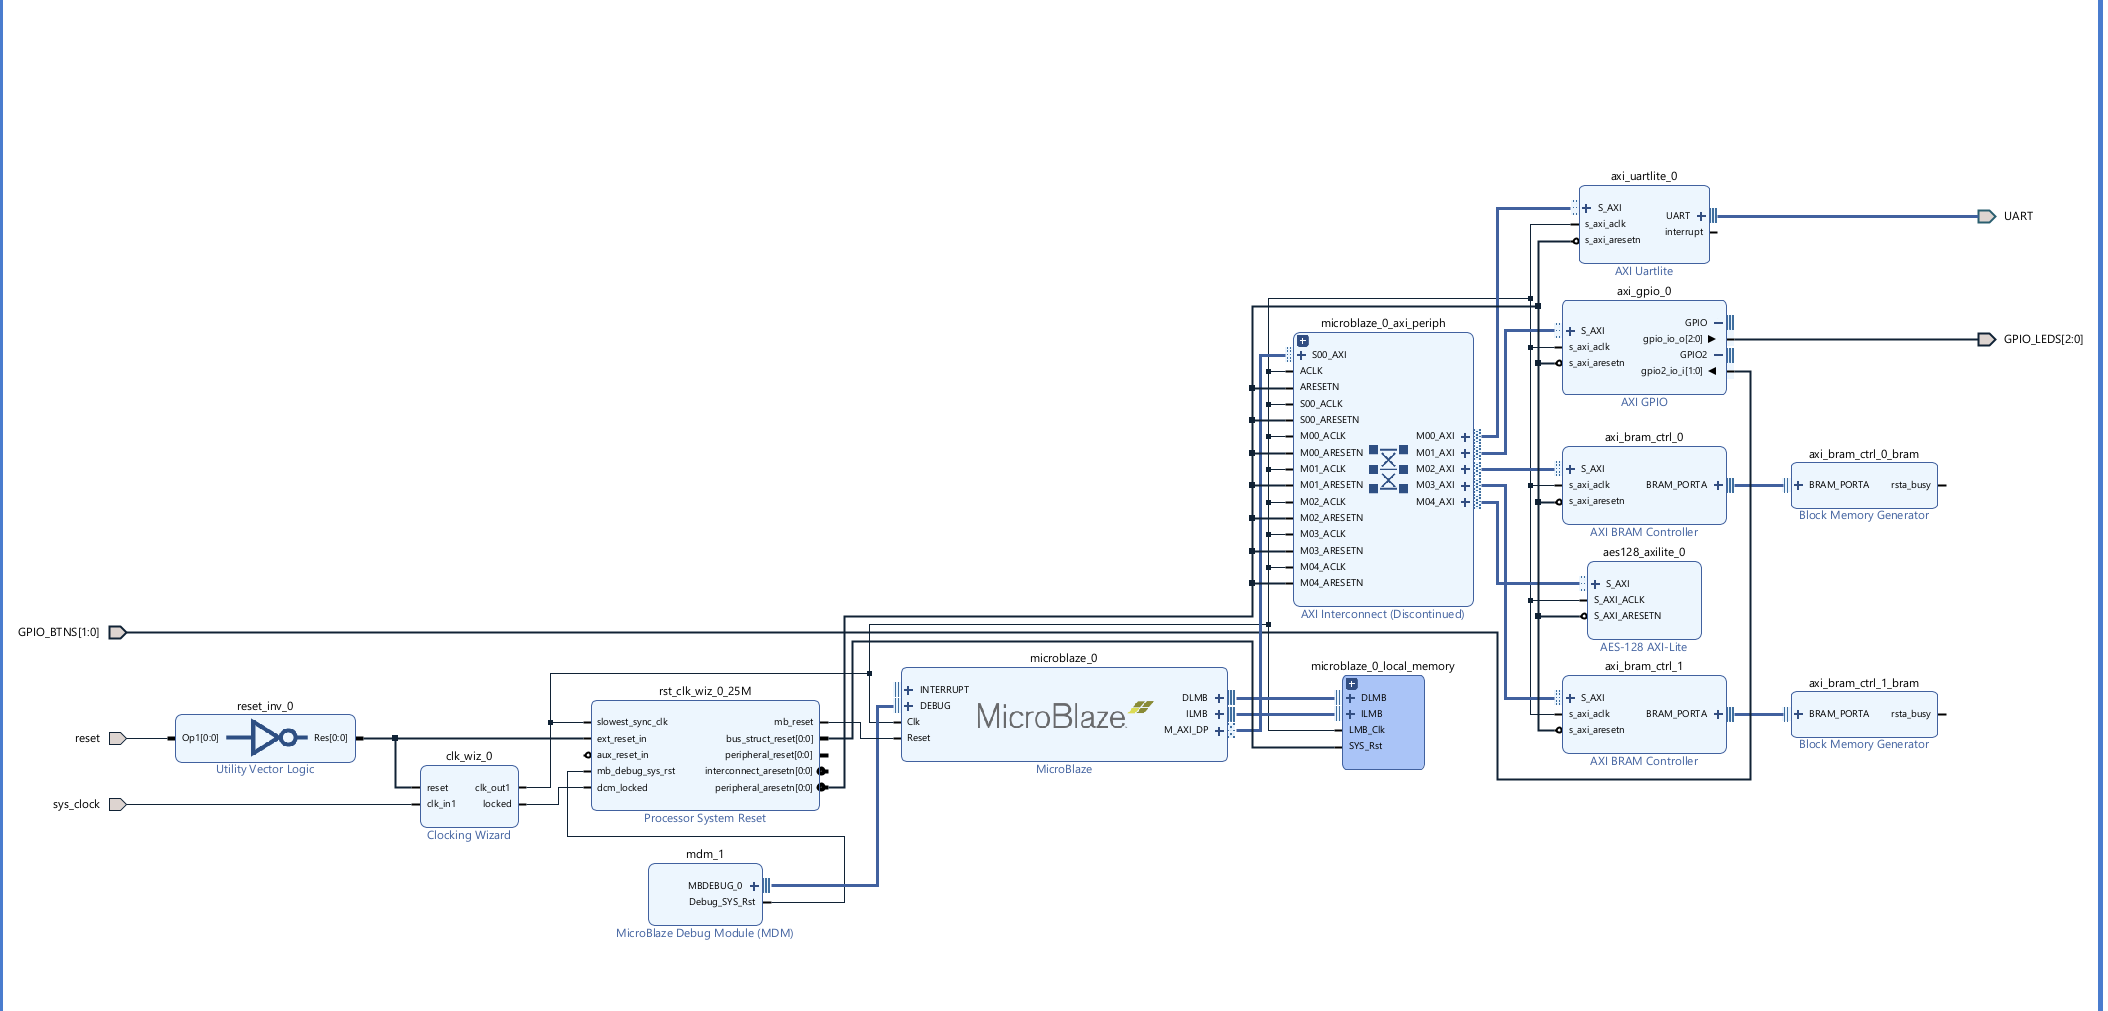
\includegraphics[width=\textwidth]{block_design.png}
    \caption{Vivado Block Design: Full SoC Architecture showing MicroBlaze, AXI Interconnect, Custom AES-128 IP, Dual BRAM Controllers, GPIO, and UART.}
    \label{fig:block_design}
\end{figure}

The architecture diagram (Figure~\ref{fig:arch_tikz}) shows the data flow from a conceptual standpoint.

\begin{figure}[H]
\centering
\begin{tikzpicture}[
    block/.style={rectangle, draw=blue!60, fill=blue!8, rounded corners, minimum width=2.8cm, minimum height=1cm, align=center, font=\small},
    memblock/.style={rectangle, draw=green!60!black, fill=green!8, rounded corners, minimum width=2.8cm, minimum height=1cm, align=center, font=\small},
    ioblock/.style={rectangle, draw=orange!70, fill=orange!8, rounded corners, minimum width=2.2cm, minimum height=0.9cm, align=center, font=\small},
    arrow/.style={-{Stealth[length=6pt]}, thick, blue!60},
    dasharrow/.style={-{Stealth[length=6pt]}, dashed, gray!70}
]

\node[block] (mb) at (0,0) {MicroBlaze\\Processor};
\node[block] (axi) at (4,0) {AXI4-Lite\\Interconnect};
\node[block] (aes) at (8,1.8) {AES-128\\IP Core};
\node[memblock] (bram0) at (8,0) {Input BRAM\\(0xC000\_0000)};
\node[memblock] (bram1) at (8,-1.8) {Output BRAM\\(0xC200\_0000)};
\node[ioblock] (gpio) at (4,2.5) {AXI GPIO\\LEDs/Buttons};
\node[ioblock] (uart) at (4,-2.5) {AXI UART\\(Bypassed)};
\node[ioblock] (jtag) at (-3,0) {JTAG/XSCT\\(Host PC)};

\draw[arrow] (mb) -- (axi);
\draw[arrow] (axi) -- (aes);
\draw[arrow] (axi) -- (bram0);
\draw[arrow] (axi) -- (bram1);
\draw[arrow] (axi) -- (gpio);
\draw[dasharrow] (axi) -- (uart);
\draw[arrow] (jtag) -- node[above, font=\tiny]{mwr/mrd} (mb);

\node[font=\tiny, text=green!50!black, align=center] at (8,0.6) {4096 bytes\\plaintext};
\node[font=\tiny, text=green!50!black, align=center] at (8,-1.1) {4096 bytes\\ciphertext};

\end{tikzpicture}
\caption{Conceptual System Architecture Block Diagram}
\label{fig:arch_tikz}
\end{figure}

\subsection{Memory Map}

\begin{table}[H]
\centering
\caption{System Memory Map}
\begin{tabular}{llll}
\toprule
\textbf{Peripheral} & \textbf{Base Address} & \textbf{Size} & \textbf{Purpose} \\
\midrule
Input BRAM (axi\_bram\_ctrl\_0)  & \texttt{0xC000\_0000} & 4 KB & Plaintext image storage \\
Output BRAM (axi\_bram\_ctrl\_1) & \texttt{0xC200\_0000} & 4 KB & Ciphertext storage \\
AES-128 IP (aes128\_axilite\_0)  & \texttt{0x44A0\_0000} & 64 B & AES register interface \\
AXI GPIO (axi\_gpio\_0)          & \texttt{0x4012\_0000} & 64 KB & LED/Button control \\
AXI UART Lite                    & \texttt{0x4060\_0000} & 64 KB & UART (bypassed) \\
\bottomrule
\end{tabular}
\end{table}

\subsection{AES-128 Core Design (\texttt{aes128\_core.v})}

The AES-128 engine is the heart of the IP core. It implements the complete FIPS-197 AES-128 ECB encryption algorithm in synthesizable Verilog-2001.

\subsubsection{Module Port Interface}

\begin{table}[H]
\centering
\caption{AES-128 Core Port Descriptions}
\begin{tabular}{llll}
\toprule
\textbf{Port} & \textbf{Direction} & \textbf{Width} & \textbf{Description} \\
\midrule
\texttt{clk}      & Input  & 1 bit  & System clock (100 MHz) \\
\texttt{rst\_n}   & Input  & 1 bit  & Active-low synchronous reset \\
\texttt{start}    & Input  & 1 bit  & Pulse HIGH for 1 cycle to begin encryption \\
\texttt{key}      & Input  & 128 bit & AES-128 encryption key \\
\texttt{data\_in} & Input  & 128 bit & Plaintext block input \\
\texttt{data\_out}& Output & 128 bit & Ciphertext block output \\
\texttt{done}     & Output & 1 bit  & Pulses HIGH for 1 cycle when output is valid \\
\bottomrule
\end{tabular}
\end{table}

\subsubsection{AES Round Operations}

The core implements all four standard AES round transformations operating on a 4$\times$4 byte state matrix:

\begin{enumerate}[leftmargin=*]
    \item \textbf{SubBytes} --- Each byte of the 128-bit state is substituted using the AES S-box, implemented as a 256-entry combinational \texttt{case} statement in Verilog. The S-box is derived from the multiplicative inverse in GF($2^8$) followed by an affine transformation.
    \item \textbf{ShiftRows} --- Row $r$ of the state matrix is cyclically shifted left by $r$ bytes (row 0: no shift, row 1: 1 byte, row 2: 2 bytes, row 3: 3 bytes), implemented as a combinational byte reorder.
    \item \textbf{MixColumns} --- Each 4-byte column is multiplied by a fixed polynomial matrix in GF($2^8$). The \texttt{xtime} function (left-shift with reduction polynomial $x^8+x^4+x^3+x+1$) is used:
    \begin{equation}
    \begin{bmatrix} r_0 \\ r_1 \\ r_2 \\ r_3 \end{bmatrix}
    =
    \begin{bmatrix} 2 & 3 & 1 & 1 \\ 1 & 2 & 3 & 1 \\ 1 & 1 & 2 & 3 \\ 3 & 1 & 1 & 2 \end{bmatrix}
    \begin{bmatrix} s_0 \\ s_1 \\ s_2 \\ s_3 \end{bmatrix}
    \pmod{x^8+x^4+x^3+x+1}
    \end{equation}
    \item \textbf{AddRoundKey} --- 128-bit XOR of the state with the current round key.
\end{enumerate}

\subsubsection{Key Expansion}

The key schedule generates 11 round keys (W[0]--W[43]) from the 128-bit input key using the \texttt{key\_expand} task. This is implemented \textbf{combinationally} and executes in the first clock cycle when \texttt{start} is asserted, using \texttt{RotWord}, \texttt{SubWord}, and the Rcon constants.

\subsubsection{Finite State Machine}

The AES core uses a simple 3-state FSM (Figure~\ref{fig:fsm_tikz}):

\begin{figure}[H]
\centering
\begin{tikzpicture}[
    state/.style={circle, draw=blue!70, fill=blue!10, thick, minimum size=2.2cm, align=center, font=\small\bfseries},
    arrow/.style={-{Stealth[length=7pt]}, thick, blue!70}
]
\node[state] (idle) at (0,0) {IDLE};
\node[state] (run) at (5,0) {RUNNING};
\node[state] (done) at (2.5,-4) {DONE};

\draw[arrow] (idle) to[bend left=20] node[above, font=\small]{start=1\\Key expand\\AddRoundKey(0)} (run);
\draw[arrow] (run) to[bend left=20] node[right, font=\small]{round $<$ 10:\\SubBytes, ShiftRows\\MixColumns, ARK} (run);
\draw[arrow] (run) to[bend left=10] node[right, font=\small]{round=10:\\SubBytes, ShiftRows, ARK} (done);
\draw[arrow] (done) to[bend left=10] node[left, font=\small]{data\_out valid\\done=1} (idle);
\end{tikzpicture}
\caption{AES Core Finite State Machine (IDLE $\to$ RUNNING $\to$ DONE)}
\label{fig:fsm_tikz}
\end{figure}

\textbf{Latency:} 12 clock cycles total --- 1 cycle for key expansion + initial AddRoundKey, 9 cycles for rounds 1--9 (with MixColumns), 1 cycle for round 10 (no MixColumns), 1 cycle to assert \texttt{done} and latch output.

\subsection{AXI4-Lite Wrapper (\texttt{aes128\_axilite\_wrapper.v})}

The AXI4-Lite wrapper exposes the AES core to the MicroBlaze processor via 14 memory-mapped 32-bit registers.

\subsubsection{AXI4-Lite Register Map}

\begin{table}[H]
\centering
\caption{AXI4-Lite Register Map (Base Address: 0x44A00000)}
\begin{tabular}{lllp{5cm}}
\toprule
\textbf{Offset} & \textbf{Register} & \textbf{R/W} & \textbf{Description} \\
\midrule
\texttt{0x00} & CTRL    & W & bit[0]=START, bit[1]=SOFT\_RST \\
\texttt{0x04} & STATUS  & R & bit[0]=DONE (latched until next START) \\
\texttt{0x08} & KEY\_W0 & W & key[127:96] \\
\texttt{0x0C} & KEY\_W1 & W & key[95:64] \\
\texttt{0x10} & KEY\_W2 & W & key[63:32] \\
\texttt{0x14} & KEY\_W3 & W & key[31:0] \\
\texttt{0x18} & DIN\_W0 & W & data\_in[127:96] \\
\texttt{0x1C} & DIN\_W1 & W & data\_in[95:64] \\
\texttt{0x20} & DIN\_W2 & W & data\_in[63:32] \\
\texttt{0x24} & DIN\_W3 & W & data\_in[31:0] \\
\texttt{0x28} & DOUT\_W0 & R & data\_out[127:96] \\
\texttt{0x2C} & DOUT\_W1 & R & data\_out[95:64] \\
\texttt{0x30} & DOUT\_W2 & R & data\_out[63:32] \\
\texttt{0x34} & DOUT\_W3 & R & data\_out[31:0] \\
\bottomrule
\end{tabular}
\end{table}

\subsection{CTR Mode Block Diagram}

Figure~\ref{fig:ctr_tikz} shows how CTR mode is implemented. The AES core encrypts a counter value (not the plaintext), and the resulting keystream is XOR'd with the plaintext to produce ciphertext --- making it a stream cipher with the security of AES.

\begin{figure}[H]
\centering
\begin{tikzpicture}[
    block/.style={rectangle, draw=blue!60, fill=blue!8, rounded corners, minimum width=2.2cm, minimum height=0.9cm, align=center, font=\small},
    xornode/.style={circle, draw=red!60, fill=red!8, minimum size=0.7cm, font=\large},
    arrow/.style={-{Stealth[length=6pt]}, thick}
]
\node[block] (ctr0) at (0,0) {CTR Block 0\\IV};
\node[block] (ctr1) at (3.5,0) {CTR Block 1\\IV+1};
\node[block] (ctr2) at (7,0) {CTR Block 2\\IV+2};
\node (dots) at (9.5,0) {\ldots};

\node[block, fill=green!8, draw=green!60] (aes0) at (0,-1.8) {AES-128\\Encrypt};
\node[block, fill=green!8, draw=green!60] (aes1) at (3.5,-1.8) {AES-128\\Encrypt};
\node[block, fill=green!8, draw=green!60] (aes2) at (7,-1.8) {AES-128\\Encrypt};

\node[xornode] (xor0) at (0,-3.6) {$\oplus$};
\node[xornode] (xor1) at (3.5,-3.6) {$\oplus$};
\node[xornode] (xor2) at (7,-3.6) {$\oplus$};

\node[above=0.4cm of xor0, font=\small] (p0) {Plain[0]};
\node[above=0.4cm of xor1, font=\small] (p1) {Plain[1]};
\node[above=0.4cm of xor2, font=\small] (p2) {Plain[2]};

\node[below=0.4cm of xor0, font=\small] (c0) {Cipher[0]};
\node[below=0.4cm of xor1, font=\small] (c1) {Cipher[1]};
\node[below=0.4cm of xor2, font=\small] (c2) {Cipher[2]};

\foreach \x in {0,1,2} {
    \pgfmathparse{int(\x*3.5)}
    \draw[arrow] (\x*3.5, -0.45) -- (\x*3.5,-1.35);
    \draw[arrow] (\x*3.5,-2.25) -- (\x*3.5,-3.25);
    \draw[arrow] (\x*3.5,-3.95) -- (\x*3.5,-4.4);
}
\draw[arrow] (p0) -- (xor0);
\draw[arrow] (p1) -- (xor1);
\draw[arrow] (p2) -- (xor2);

\end{tikzpicture}
\caption{AES-128 CTR Mode Operation: Counter blocks are encrypted to generate a keystream, which is XOR'd with plaintext blocks to produce ciphertext.}
\label{fig:ctr_tikz}
\end{figure}
